{\em Equal Sudoku} ist eine Variante des bekannten Sudoku, in dem 
einige Felder zusätzlich eingefärbt sind.
Die Lösungszahlen in jedem zusammenhängenden farbigen Gebiet müssen die
folgenden zusätzlichen Bedingungen erfüllen:
\begin{enumerate}
\item
Die Summe der geraden Zahlen und die Summe der ungeraden Zahlen müssen
gleich sein.
\item 
In einem farbigen Gebiet darf keine Zahl zweimal vorkommen.
\end{enumerate}
Das erstaunliche ist, dass die Lösung eines solchen {\em Equal Sudoku}
mit wesentlich weniger Vorgaben auskommt.

\begin{center}
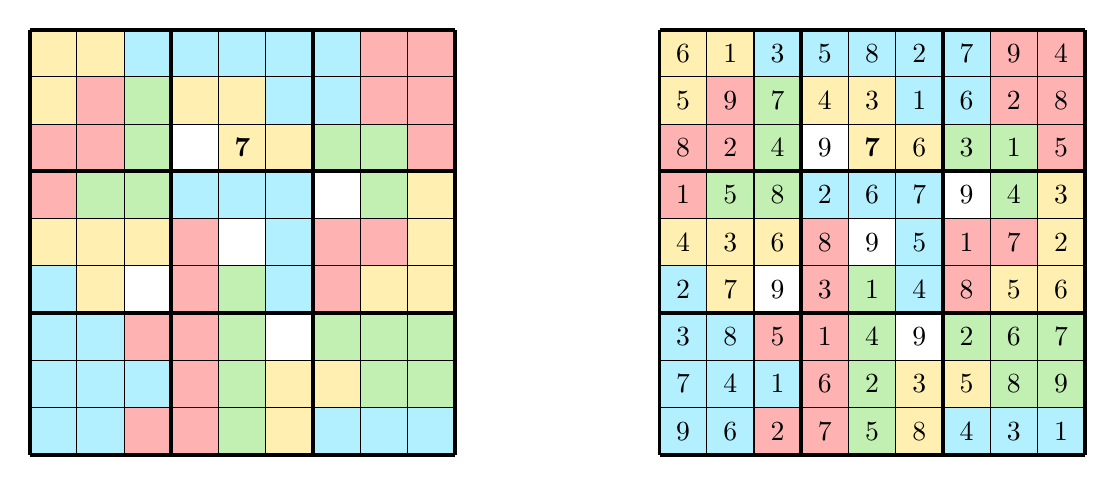
\begin{tikzpicture}[>=latex,thick]
\def\gs{0.6}

\def\farbfeld#1#2#3{
	\fill[color=#3!30]
		({(#1-1)*\gs},{(#2-1)*\gs}) rectangle ({(#1)*\gs},{(#2)*\gs});
}

\def\zahlfeld#1#2#3{
	\node at ({(#1-0.5)*\gs},{(#2-0.5)*\gs}) {$#3$};
}

\def\gitter{
	\foreach \x in {0,...,9}{
		\draw[line width=0.4pt] ({\x*\gs},{0*\gs})--({\x*\gs},{9*\gs});
	}
	\foreach \x in {0,3,...,9}{
		\draw[line width=1.4pt] ({\x*\gs},{0*\gs})--({\x*\gs},{9*\gs});
	}
	\foreach \y in {0,...,9}{
		\draw[line width=0.4pt] ({0*\gs},{\y*\gs})--({9*\gs},{\y*\gs});
	}
	\foreach \y in {0,3,...,9}{
		\draw[line width=1.4pt] ({0*\gs},{\y*\gs})--({9*\gs},{\y*\gs});
	}
}

\definecolor{blau}{rgb}{0,0.8,1}
\definecolor{rot}{rgb}{1,0,0}
\definecolor{gruen}{rgb}{0.2,0.8,0}
\definecolor{gelb}{rgb}{1.0,0.8,0}
\definecolor{magenta}{rgb}{1.0,1.0,1.0}

\def\farben{
	\farbfeld{1}{1}{blau}
	\farbfeld{2}{1}{blau}
	\farbfeld{3}{1}{rot}
	\farbfeld{4}{1}{rot}
	\farbfeld{5}{1}{gruen}
	\farbfeld{6}{1}{gelb}
	\farbfeld{7}{1}{blau}
	\farbfeld{8}{1}{blau}
	\farbfeld{9}{1}{blau}

	\farbfeld{1}{2}{blau}
	\farbfeld{2}{2}{blau}
	\farbfeld{3}{2}{blau}
	\farbfeld{4}{2}{rot}
	\farbfeld{5}{2}{gruen}
	\farbfeld{6}{2}{gelb}
	\farbfeld{7}{2}{gelb}
	\farbfeld{8}{2}{gruen}
	\farbfeld{9}{2}{gruen}

	\farbfeld{1}{3}{blau}
	\farbfeld{2}{3}{blau}
	\farbfeld{3}{3}{rot}
	\farbfeld{4}{3}{rot}
	\farbfeld{5}{3}{gruen}
	\farbfeld{6}{3}{magenta}
	\farbfeld{7}{3}{gruen}
	\farbfeld{8}{3}{gruen}
	\farbfeld{9}{3}{gruen}

	\farbfeld{1}{4}{blau}
	\farbfeld{2}{4}{gelb}
	\farbfeld{3}{4}{magenta}
	\farbfeld{4}{4}{rot}
	\farbfeld{5}{4}{gruen}
	\farbfeld{6}{4}{blau}
	\farbfeld{7}{4}{rot}
	\farbfeld{8}{4}{gelb}
	\farbfeld{9}{4}{gelb}

	\farbfeld{1}{5}{gelb}
	\farbfeld{2}{5}{gelb}
	\farbfeld{3}{5}{gelb}
	\farbfeld{4}{5}{rot}
	\farbfeld{5}{5}{magenta}
	\farbfeld{6}{5}{blau}
	\farbfeld{7}{5}{rot}
	\farbfeld{8}{5}{rot}
	\farbfeld{9}{5}{gelb}

	\farbfeld{1}{6}{rot}
	\farbfeld{2}{6}{gruen}
	\farbfeld{3}{6}{gruen}
	\farbfeld{4}{6}{blau}
	\farbfeld{5}{6}{blau}
	\farbfeld{6}{6}{blau}
	\farbfeld{7}{6}{magenta}
	\farbfeld{8}{6}{gruen}
	\farbfeld{9}{6}{gelb}

	\farbfeld{1}{7}{rot}
	\farbfeld{2}{7}{rot}
	\farbfeld{3}{7}{gruen}
	\farbfeld{4}{7}{magenta}
	\farbfeld{5}{7}{gelb}
	\farbfeld{6}{7}{gelb}
	\farbfeld{7}{7}{gruen}
	\farbfeld{8}{7}{gruen}
	\farbfeld{9}{7}{rot}

	\farbfeld{1}{8}{gelb}
	\farbfeld{2}{8}{rot}
	\farbfeld{3}{8}{gruen}
	\farbfeld{4}{8}{gelb}
	\farbfeld{5}{8}{gelb}
	\farbfeld{6}{8}{blau}
	\farbfeld{7}{8}{blau}
	\farbfeld{8}{8}{rot}
	\farbfeld{9}{8}{rot}

	\farbfeld{1}{9}{gelb}
	\farbfeld{2}{9}{gelb}
	\farbfeld{3}{9}{blau}
	\farbfeld{4}{9}{blau}
	\farbfeld{5}{9}{blau}
	\farbfeld{6}{9}{blau}
	\farbfeld{7}{9}{blau}
	\farbfeld{8}{9}{rot}
	\farbfeld{9}{9}{rot}
}

\begin{scope}[xshift=-4cm]
\farben
\zahlfeld{5}{7}{\mathbf{7}}
\gitter
\end{scope}

\begin{scope}[xshift=4cm]
\farben
\zahlfeld{1}{1}{9}
\zahlfeld{2}{1}{6}
\zahlfeld{3}{1}{2}
\zahlfeld{4}{1}{7}
\zahlfeld{5}{1}{5}
\zahlfeld{6}{1}{8}
\zahlfeld{7}{1}{4}
\zahlfeld{8}{1}{3}
\zahlfeld{9}{1}{1}

\zahlfeld{1}{2}{7}
\zahlfeld{2}{2}{4}
\zahlfeld{3}{2}{1}
\zahlfeld{4}{2}{6}
\zahlfeld{5}{2}{2}
\zahlfeld{6}{2}{3}
\zahlfeld{7}{2}{5}
\zahlfeld{8}{2}{8}
\zahlfeld{9}{2}{9}

\zahlfeld{1}{3}{3}
\zahlfeld{2}{3}{8}
\zahlfeld{3}{3}{5}
\zahlfeld{4}{3}{1}
\zahlfeld{5}{3}{4}
\zahlfeld{6}{3}{9}
\zahlfeld{7}{3}{2}
\zahlfeld{8}{3}{6}
\zahlfeld{9}{3}{7}

\zahlfeld{1}{4}{2}
\zahlfeld{2}{4}{7}
\zahlfeld{3}{4}{9}
\zahlfeld{4}{4}{3}
\zahlfeld{5}{4}{1}
\zahlfeld{6}{4}{4}
\zahlfeld{7}{4}{8}
\zahlfeld{8}{4}{5}
\zahlfeld{9}{4}{6}

\zahlfeld{1}{5}{4}
\zahlfeld{2}{5}{3}
\zahlfeld{3}{5}{6}
\zahlfeld{4}{5}{8}
\zahlfeld{5}{5}{9}
\zahlfeld{6}{5}{5}
\zahlfeld{7}{5}{1}
\zahlfeld{8}{5}{7}
\zahlfeld{9}{5}{2}

\zahlfeld{1}{6}{1}
\zahlfeld{2}{6}{5}
\zahlfeld{3}{6}{8}
\zahlfeld{4}{6}{2}
\zahlfeld{5}{6}{6}
\zahlfeld{6}{6}{7}
\zahlfeld{7}{6}{9}
\zahlfeld{8}{6}{4}
\zahlfeld{9}{6}{3}

\zahlfeld{1}{7}{8}
\zahlfeld{2}{7}{2}
\zahlfeld{3}{7}{4}
\zahlfeld{4}{7}{9}
\zahlfeld{5}{7}{\mathbf{7}}
\zahlfeld{6}{7}{6}
\zahlfeld{7}{7}{3}
\zahlfeld{8}{7}{1}
\zahlfeld{9}{7}{5}

\zahlfeld{1}{8}{5}
\zahlfeld{2}{8}{9}
\zahlfeld{3}{8}{7}
\zahlfeld{4}{8}{4}
\zahlfeld{5}{8}{3}
\zahlfeld{6}{8}{1}
\zahlfeld{7}{8}{6}
\zahlfeld{8}{8}{2}
\zahlfeld{9}{8}{8}

\zahlfeld{1}{9}{6}
\zahlfeld{2}{9}{1}
\zahlfeld{3}{9}{3}
\zahlfeld{4}{9}{5}
\zahlfeld{5}{9}{8}
\zahlfeld{6}{9}{2}
\zahlfeld{7}{9}{7}
\zahlfeld{8}{9}{9}
\zahlfeld{9}{9}{4}

\gitter
\end{scope}

\end{tikzpicture}
\end{center}
Kann eine nichtdeterministische Turing-Maschine in polynomieller 
Zeit entscheiden, ob ein {\em Equal Sudoku} eine Lösung hat?

\thema{NP}
\thema{polynomieller Verifizierer}

\begin{loesung}
Das Problem ist sicher entscheidbar, man kann alle Belegungen des Feldes
mit Zahlen durchprobieren, ob sie alle Bedingungen erfüllen.

Um zu zeigen, dass das Problem in NP ist, müssen wir zeigen, dass es in
polynomieller Zeit verifizierbar ist.
Als Lösungszertifikat verwenden wird die Lösungszahlen für alle Felder.
Der Verifikationsalgorithmus muss dann zunächst prüfen, ob die bekannten
Sudoku-Regeln in erfüllt sind, dies ist aber sicher in polynomieller
Zeit möglich, da wir ja schon wissen, dass Sudoku in NP ist.

Wie bei Sudoku üblich bezeichnen wir die Seitenlänge der Unterquadrate mit $n$,
das Spielfeld hat also $n^2\times n^2=n^4$ Felder.
Es sind jetzt also die folgenden zusätzlichen Verifikationen auszuführen:
\begin{center}
\begin{tabular}{l|p{12cm}|>{$}c<{$}}
&Verifikationsschritt&\text{Laufzeit}
\\
\hline
1&Für jedes farbige Gebiet ermittle die Felder gleicher Farbe, da dazu
gehören.
	&O(n^4)\phantom{\mathstrut\times O(n^4)}
\\
1.1&In jedem farbigen Feld bestimme die Summe der geraden und
ungeraden Zahlen und prüfe, ob sie gleich sind.
Für jedes so gefundene farbige Gebiet, verifiziere die folgenden zwei
Eigenschaften.
	&\phantom{O(n^4)}\mathstrut \times O(n^4)
\\
1.2&In jedem farbigen Gebiet überprüfe, dass jede Zahl höchstens einmal
vorkommt
	&\phantom{O(n^4)}\mathstrut \times O(n^4)
\\
\hline
&Total& \phantom{O(n^4)\times\mathstrut} O(n^8)
\\
\hline
\end{tabular}
\end{center}
Alle Verifikationen sind also in polynomieller Zeit möglich.
Damit haben wir einen polynomiellen Verifizierer gefunden was beweist,
dass das Problem in NP ist.
\end{loesung}

\begin{diskussion}
{\em Equal Sudoku} wurde von Christoph Seeliger entwickelt, das vorgestellte
Beispiel wird von {\em Cracking the Cryptic} in diesem Video
\url{https://www.youtube.com/watch?v=ygCqTawsmsM}
live gelöst.
\end{diskussion}

\begin{bewertung}
Entscheidbarkeit ({\bf E}) 1 Punkt,
Verifizierer ({\bf V}) 1 Punkt,
Zertifikat ({\bf Z}) 1 Punkt,
Verifikation von zwei zusätzlichen Regeln ({\bf R}) 2 Punkt,
Laufzeit polynomiell ({\bf L}) 1 Punkt.
\end{bewertung}

